\documentclass[border=2mm]{standalone}
\usepackage{amsmath}
\usepackage{tikz}
\usetikzlibrary{arrows.meta,positioning}
% SCHEME COLOR: one mid-grey for both GitHub light and dark themes
\definecolor{schemeink}{HTML}{808080}
\tikzset{every picture/.append style={color=schemeink}}
\newcommand{\Lext}{\mathbf{L}^{\mathrm{e}}}
\newcommand{\Lapri}{\mathbf{L}^{\mathrm{a}}}
\begin{document}
% Alternative A — Minimal / academic (Forney-style)
% Thin lines, no fills, sharp corners, math-italic block labels.
% Compactness pass: minimum height 12mm, minimum width 17mm, inner sep 4pt.
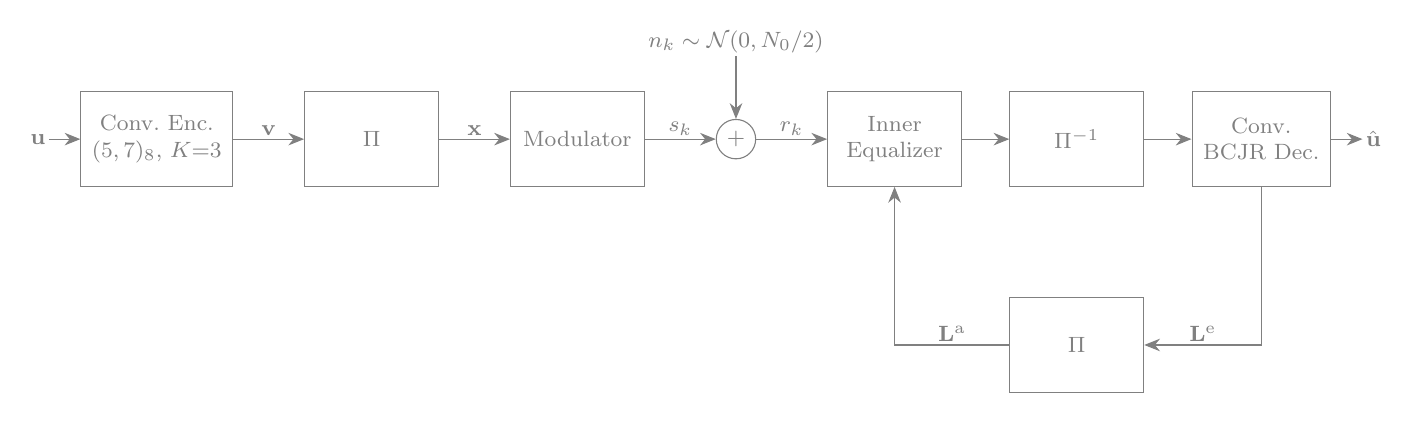
\begin{tikzpicture}[
  >={Stealth[length=2mm,width=1.6mm]},
  every path/.style={line width=0.4pt},
  block/.style={draw, line width=0.4pt,
                minimum height=12mm, minimum width=17mm,
                inner sep=4pt, align=center, font=\footnotesize},
  sum/.style={draw, circle, inner sep=0pt, minimum size=5mm,
              font=\footnotesize},
  signal/.style={font=\footnotesize, inner sep=1pt},
]
% --- Forward chain (left to right) ---
\node[signal] (u) {$\mathbf{u}$};
\node[block, right=4mm of u]   (enc) {Conv.\ Enc.\\$(5,7)_8$, $K{=}3$};
\node[block, right=9mm of enc] (pif) {$\Pi$};
\node[block, right=9mm of pif] (mod) {Modulator};
\node[sum,   right=9mm of mod] (ch)  {$+$};
\node[block, right=9mm of ch]  (eq)  {Inner\\Equalizer};
\node[block, right=6mm of eq]  (dpi) {$\Pi^{-1}$};
\node[block, right=6mm of dpi] (dec) {Conv.\\BCJR Dec.};
\node[signal, right=4mm of dec] (uhat) {$\hat{\mathbf{u}}$};

% --- Forward arrows with sequence labels ---
\draw[->] (u)   -- (enc);
\draw[->] (enc) -- node[above, signal]{$\mathbf{v}$} (pif);
\draw[->] (pif) -- node[above, signal]{$\mathbf{x}$} (mod);
\draw[->] (mod) -- node[above, signal]{$s_k$} (ch);
\draw[->] (ch)  -- node[above, signal]{$r_k$} (eq);
\draw[->] (eq)  -- (dpi);
\draw[->] (dpi) -- (dec);
\draw[->] (dec) -- (uhat);

% --- Noise input to AWGN block ---
\node[signal, above=8mm of ch] (n) {$n_k \sim \mathcal{N}(0, N_0/2)$};
\draw[->] (n) -- (ch);

% --- Feedback path: re-interleaver below the main row ---
\node[block, below=14mm of dpi] (rpi) {$\Pi$};

% L^e: decoder south, down then left into re-interleaver east
\coordinate (fb_dec_corner) at (dec.south |- rpi.east);
\draw[->] (dec.south) -- (fb_dec_corner)
                       -- node[above, signal]{$\Lext$} (rpi.east);

% L^a: re-interleaver west, left then up into equalizer south
\coordinate (fb_eq_corner) at (eq.south |- rpi.west);
\draw[->] (rpi.west) -- node[above, signal]{$\Lapri$} (fb_eq_corner)
                     -- (eq.south);
\end{tikzpicture}

\end{document}
